\documentclass[a4paper,11pt]{article}

\title{MA4J5:Structures of Complex Systems Project \\
Image Recognition for Handwriting with Tensorflow}
\author{Aadam Ul Haq \\
u2001509}
\date{\today} % leaving the braces empty surpresses the date.  You could instead manually input a date or use \date{\today}

% Now I specify packages fo code I will need that aren't standard.

% the first three packages are the used extensively in maths.
\usepackage{amsmath} 
\usepackage{amsfonts}
\usepackage{amssymb}


\usepackage{framed} % to create boxes around text using \begin{framed}....\end{framed}
\usepackage{pifont} % to allow windings, such as \ding{125} which created the oversized quotation mark
\usepackage{enumerate} % to allow customisable numbered lists
\usepackage{wasysym} % to make the arrow symbol \pointer used here as a bullet
\usepackage[super]{nth} % to use \nth commands for superscripts on ordinals
\usepackage{amsthm} %  package used to make the theorem environments work.

\theoremstyle{plain} % this sets the style for all new environments created using \newtheorem to have the "theorem" style, which as a bold title, italic text and vertical space above and below it. 
\newtheorem{thm}{Theorem}[section] 
\newtheorem{lem}[thm]{Lemma} 
\newtheorem{prop}[thm]{Proposition} 
\newtheorem*{cor}{Corollary} 
\newtheorem*{claim}{Claim} 

\theoremstyle{definition} % this sets the style for all new environments created using \newtheorem to have the "definition" style, which as a bold title, upright text and vertical space above and below it.
\newtheorem{defn}{Definition}[section]
\newtheorem{eg}{Example}[section]


\theoremstyle{remark} % this sets the style for all new environments created using \newtheorem to have the "remark" style, which as an italic non-bold title, upright text and no extra vertical space above and below it.
\newtheorem*{rem}{Remark} 
\newtheorem{case}{Case}

% packages needed for the bibliography to work nicely:
\usepackage[numbers]{natbib}
\bibliographystyle{plainnat}
\usepackage{cite}

\usepackage{url}% allows use of the \url{...} command to typeset a url properly
\usepackage{graphicx}
\usepackage{listings}

\usepackage{xurl}
\usepackage{breakurl}
\usepackage{hyperref}
\usepackage{cleveref}

\begin{document}  

\maketitle  
\begin{abstract}
Image recognition is a useful tool within Artificial Intelligence. It is a tool within Deep Learning, which is a subset within Machine Learning. In this report, we will examine handwritten digit recognition within Python, using the package `Tensorflow', creating a neural network and analysing the performances of the models.
\end{abstract}
\tableofcontents 

\pagebreak

\section{Introduction and Mathematical Backgorund}

\subsection{Overview of Artificial Intelligence}

Machine Learning (ML) is a subset of Artificial Intelligence. Artificial Intelligence comprise any technique that make computers `smart', mimicking human behavior; whereas Machine Learning utilise statistical methods to enable computers the capacity to learn without being explicitly programmed. Artificial Intelligence that is not Machine Learning is often known as GOFAI (Good Old-Fashioned Artificial Intelligence). The most renowned example of this is an AI Chatbox, SHRDLU developed by Terry Winograd at MIT in $1968$. This contributed greatly to  major advancements in the evolution of Neural Linguistic Programming. It is smart but has no
ability to learn as it relies only on a set of human-defined
rules to reply to customer questions within a limited domain. In contrast, Machine Learning can be used in things such as robots; unlike SHRDLU, a robot can `learn' from its past mistakes, as shown in Boston Dynamics' robot, Atlas.

Neural Computing is a further subset of Machine Learning that uses brain inspired Machine Learning techniques that use neural networks. An example of Machine Learning that is not Neural Computing would be Support Vector Machine (SVM). This is an ML algorithm that
does not use networks of
neurons  and is used for data classification to maximally separate different classes in  training data. Finally, Deep Learning is a subset of Neural Computing which uses deep neural networks to build a hierarchy of data representations. Typically, Deep Learning methods are defined as algorithms that are trained on
multi-layer neural networks with three or more layers.

A key distinction between the types of Artificial Intellegence is the way the data is given. The main distinctions between Machine Learning and Neural Computing are summarised in Table \ref{Table1}.
\begin{table}[htb]
    \centering
        \begin{tabular}{ |l | c c|} 
            \hline
             & Machine Learning & Neural Computing \\ 
            \hline
            Features Chosen by Human?         & Yes & No \\ 
            Training Data & Small & Large \\ 
            Training Time       & Short & Long \\ 
            Accuracy      & Low & High \\ 
            \hline
        \end{tabular}%
    \caption{Differences between Machine Learning and Neural Computing}
    \label{Table1}
\end{table}
An example of the differences between the two can be shown in recognising cars in an image. If we used Machine Learning, we would have to provide a training set with labelled data. This data would have many examples of cars and many examples of things that are not cars. Once the computer has learned the data, we can test it on a testing set. For neural computing, we do not need to label our data as the model learns what the car is itself.

\subsection{How Neural Networks Learn}

Neural networks are built from units called perceptrons. Perceptrons fire if a certain linear combination of inputs, $\boldsymbol{w}^T \boldsymbol{x}$, exceeds a threshold $-b$. 
This is the similar to solving the problem of binary classification using a linear function. Given a vector of weights $\boldsymbol{w} \in \mathbb{R}^d$, input vectors $\boldsymbol{x} \in \mathbb{R}^d$ and a bias term $b \in \mathbb{R}$, the binary classifier would give the output,
$$
h_{\boldsymbol{w}, b}(\boldsymbol{x})= g(\boldsymbol{x}) = \mathbf{1}\left\{\boldsymbol{w}^T \boldsymbol{x}+b>0\right\}= \begin{cases}1 & \boldsymbol{w}^T \boldsymbol{x}+b>0 \\ 0 & \boldsymbol{w}^T \boldsymbol{x}+b \leq 0\end{cases}
$$
In this case, $g(\boldsymbol{x})$ is chosen to be the the indicator function, $\mathbf{1}$. The choice of function for $g(\boldsymbol{x})$ is known as the activation function. There are many possible functions that can be chosen. One of the most common choices is the sigmoid function.
In order to determine the weights and bias term from data using optimization, it is useful to approximate the indicator with a smooth function such as the sigmoid
$$
\sigma(x)=\frac{1}{1+\mathrm{e}^{-x}} .
$$

The most desirable feature of activation functions are that they are easily differentiable and are smooth. This makes backpropogation easier to calculate the weights and biases.

Neural Networks are built from layers of perceptrons with connections between the current and next layer.
We define a linear $\operatorname{map} \boldsymbol{W}^k: \mathbb{R}^{d_{k-1}} \rightarrow \mathbb{R}^{d_k}$ and a bias vector $\boldsymbol{b}^k \in \mathbb{R}^{d_k}$, to the $k$-th layer where $d_k$ are the number of perceptrons in layer $k$. Applying an activation function componentwise (in this case the sigmoid activation was chosen for simplicity), we obtain a map,
$
\sigma\left(\boldsymbol{W}^k \boldsymbol{x}+\boldsymbol{b}^k\right)
$ from layer $k-1$ to $k$.

The first layer is the input layer, while the last layer is the output layer. Hence, a neural network with $\ell$ layers is a function of the form $F^{\ell}(\boldsymbol{x})$, where the $F^k$ are recursively defined as
$$
\begin{aligned}
F^1(\boldsymbol{x}) & =\sigma\left(\boldsymbol{W}^1 \boldsymbol{x}+\boldsymbol{b}^1\right) \\
F^{k+1}(\boldsymbol{x}) & =\sigma\left(\boldsymbol{W}^{(k+1)} F^k(\boldsymbol{x})+\boldsymbol{b}^{k+1}\right), \quad 1 \leq k<\ell,
\end{aligned}
$$
and $\boldsymbol{W}^k \in \mathbb{R}^{d_k \times d_{k-1}}, \boldsymbol{b}^k \in \mathbb{R}^{d_k}$ for $1 \leq k \leq \ell$ (with $d_0=d$ ). The layers between the input and output layer are called the hidden layers. Different hidden layers may have different activation functions. Such a set of specifications defines what is called an architecture such as in Figure \cref{AI}.

\begin{figure}[htb]
	\centering 
	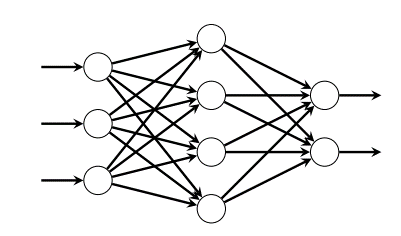
\includegraphics[width=0.45\textwidth, angle=0]{Picture1.png}	
	\caption{Neural Network Architecture.  Each layer corresponds to a linear map of the outputs of the
previous layer, followed by an activation function. Each arrow represents a weight.} 
	\label{AI}%
\end{figure}

We can train a neural network on data $\left(\boldsymbol{x}_i, \boldsymbol{y}_i\right), i \in\{1, \ldots, n\}$, by minimizing the empirical risk, $
\hat{R}(h)$, with respect to a loss function, $L\left(h\left(\boldsymbol{x}^i\right), \boldsymbol{y}^i\right)$. The empirical risk of a function $h: \mathcal{X} \rightarrow \mathcal{Y}$ is the average loss over the training data,
$
\hat{R}(h):=\frac{1}{n} \sum_{i=1}^n L\left(h\left(\boldsymbol{x}^i\right), \boldsymbol{y}^i\right)
$. $L$ is a loss function, of which there are many possibilities. A loss function $L: \mathcal{Y} \times \mathcal{Y} \rightarrow \mathbb{R}_{+}$measures the mismatch between a prediction on a given input $\boldsymbol{x} \in \mathcal{X}$ and an element $\boldsymbol{y} \in \mathcal{Y}$. 

To minimise the empirical risk, if $L$ is differentiable almost everywhere, then the method of choice is gradient descent, using a computational implementation of the chain rule known as backpropagation. Firstly a few definitions must be made. 

Denote $\boldsymbol{W}$ and $\boldsymbol{b}$ as the concatenation of all the weight matrices and bias vectors. We denote $w_{i j}^k$ the $(i, j)$-th entry of the $k$-th matrix, and $b_i^k$ the $i$-th entry of the $k$-th bias vector. The aim is then to minimize the empirical risk,
$
f(\boldsymbol{W}, \boldsymbol{b}):=\frac{1}{n} \sum_{i=1}^n L\left(F^{\ell}\left(\boldsymbol{x}_i\right), \boldsymbol{y}_i\right) .
$.

Gradient descent, or stochastic gradient descent, requires evaluating the gradient of a function of the form
$$
f_i(\boldsymbol{W}, \boldsymbol{b}):=L\left(F^{\ell}\left(\boldsymbol{x}_i\right), \boldsymbol{y}_i\right) .
$$

Setting $\boldsymbol{x}=\boldsymbol{x}_i$ and $\boldsymbol{y}=\boldsymbol{y}_i$, and also writing $\boldsymbol{a}^0:=\boldsymbol{x}$,  for $k \in\{1, \ldots, \ell\}$ we let
$
\boldsymbol{z}^k=\boldsymbol{W}^k \boldsymbol{a}^{k-1}+\boldsymbol{b}^k, \quad \boldsymbol{a}^k=\sigma\left(\boldsymbol{z}^k\right) .
$
In particular, $\boldsymbol{a}^{\ell}=F^{\ell}(\boldsymbol{x})$ is the output of the neural network on input $\boldsymbol{x}$. 

Moreover, set $C=C(\boldsymbol{W}, \boldsymbol{b})=$ $L\left(\boldsymbol{a}^{\ell}, \boldsymbol{y}\right)$ for the loss function.
For every layer $k$ and coordinate $j \in\left\{1, \ldots, d_k\right\}$, the sensitivities are defined as
$$
\delta_j^k:=\frac{\partial C}{\partial z_j^k},
$$
where $z_j^k$ is the $j$-th coordinate of $z^k$. Thus $\delta_j^k$ measures the sensitivity of the loss function to the input at the $j$-th node of the $k$-th layer. Denote $\boldsymbol{\delta}^k \in \mathbb{R}^{d_k}$ the vector of $\delta_j^k$ for $j \in\left\{1, \ldots, d_k\right\}$. The partial derivatives of $C$ can be computed in terms of these quantities.


\begin{thm}[Backpropogation] For a neural network with $\ell$ layers and $k \in\{1, \ldots, \ell\}$, we have
$$
\frac{\partial C}{\partial w_{i j}^k}=\delta_i^k a_j^{k-1}, \quad \frac{\partial C}{\partial b_i^k}=\delta_i^k
$$
for $i, j \in\left\{1, \ldots, d_k\right\}$. Moreover, the sensitivities $\delta_i^k$ can be computed as follows:
$$
\boldsymbol{\delta}^{\ell}=\sigma^{\prime}\left(\boldsymbol{z}^{\ell}\right) \circ \nabla_{\boldsymbol{a}^{\ell}} L\left(\boldsymbol{a}^{\ell}, \boldsymbol{y}\right), \quad \boldsymbol{\delta}^k=\sigma^{\prime}\left(\boldsymbol{z}^k\right) \circ\left(\boldsymbol{W}^{k+1}\right)^T \boldsymbol{\delta}^{k+1}
$$
for $k \in\{1, \ldots, \ell-1\}$.
\end{thm}

A proof can be found in \Citet{higham2019deep}. Once the weights and biases are learned using the backpropogation technique, the neural network can be tested on test data. 

\subsection{Image Recognition}

Character and digit recognition are very well-studied problems and are often used to test new machine learning models. In particular, the
MNIST (Modified National Institute of Standards and Technology) dataset is often used and is the dataset that will be used in this report. 

Within the research community, handwriting recognition has
two different forms: offline recognition and online recognition. Offline recognition is written on media such as paper and then scanned, whereas online recognition is performed digitally. Online recognition has a higher accuracy due to additional information that can be obtained such as pen strokes. However the dataset used in this report is offline data. Offline
handwriting recognition is used in large-scale real-world
systems such as interpreting handwritten postal addresses
or monetary values on bank cheques, so research to improve performance is constantly conducted \citep{kukreja2022machine}.

Due to the constant use of handwriting datasets being used to test machine learning models, many different approaches can be used such as Convolutional Neural Networks, basic Ensemble Algorithms and new Reinforcement Learning Techniques. The purpose of the report is to evaluate a few of these models and compare how they perform.

\section{Data Preprocessing}

The MNIST dataset is built within Tensorflow in Python. It is a dataset with $60,000$ training images with their labels, and testing data with $10,000$ values. All images have a handwritten number from $0-9$, creating $10$ different classes as shown in Figure \cref{MNIST}.

Before training a neural network, data preprocessing must be conducted and an architecture must be chosen for the neural network.

\begin{figure}[htb]
	\centering 
	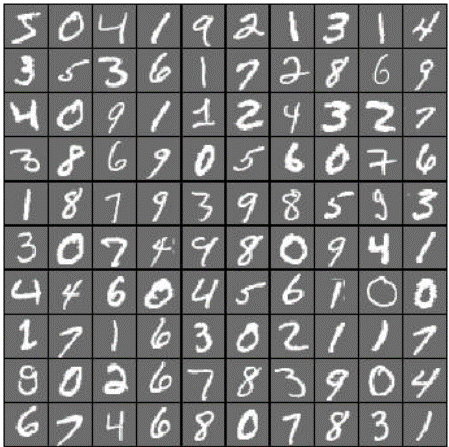
\includegraphics[width=0.45\textwidth, angle=0]{Picture2.png}	
	\caption{Example of some images within the MNIST dataset.} 
	\label{MNIST}%
\end{figure}
\subsection{Scaling}

In order for our model to read the data, we must convert the data into a readable format. Each digit is formatted in a $28$x$28$ pixel square. Each pixel also has a value between $0$ and $255$, with $0$ indicating the colour white, $255$ being black, and integers inbetween representing various shades of gray. 

For the neural network to run well, firstly each pixel is divided by $255$ to obtain a number between $0$ and $1$. This normalisation reduces the distance between the numbers and is helpful as neural networks process inputs using small weight values, and inputs with large integer values can disrupt or slow down the learning process. We then reshape the image into $784$ row vectors ($28^2$) with each representing one pixel. This is known as flattening the image.

Finally, for our labels, it helps the neural network if we `one-hot encode' our values. As our labels are the digits $0-9$, the vector contains ten values, one for each possible digit. One-hot encoding involves setting a value in our vector to $1$ and the rest are $0$ to represent the digit at the index of the vector. For example, the digit $7$ is represented using the vector $[0, 0, 0, 0, 0, 0, 0, 1, 0, 0]$ as the value at index $7$ is stored as $1$.

\subsection{Architecture}

The architecture of our neural network can vary drastically. The performance can be thought of as a function of the architecture among other things, such as the parameters, the data, and the duration of training. We will test several variations of our network to find which performs the best. Every network begins and ends in the same fashion: we must have $784$ input nodes and $10$ output nodes. These represent each of our pixels and each of our $10$ possibilities for numbers respectively. 

The variables that we can alter are:
\begin{enumerate}
    \item The number of hidden layers we have (more hidden layers makes our neural network `deeper')
    \item The number of nodes in each hidden layer. Often these increase over time to form a pyramid shape and can be effective in capturing hierarchical features.
    \item The activation function in each hidden layer. We will use sigmoid as defined earlier, and $\operatorname{ReLU}(X)=\operatorname{max}(0,X)$
    \item The optimizers and loss functions. The optimizers used are \texttt{SGD} (Stochastic Gradient Descent) and \texttt{Adam} (Adaptive Moment Estimation). The losses used are \texttt{categorical\_crossentropy} and \texttt{mean\_absolute\_error}.

\end{enumerate}

\begin{figure}[htb]
	\centering 
	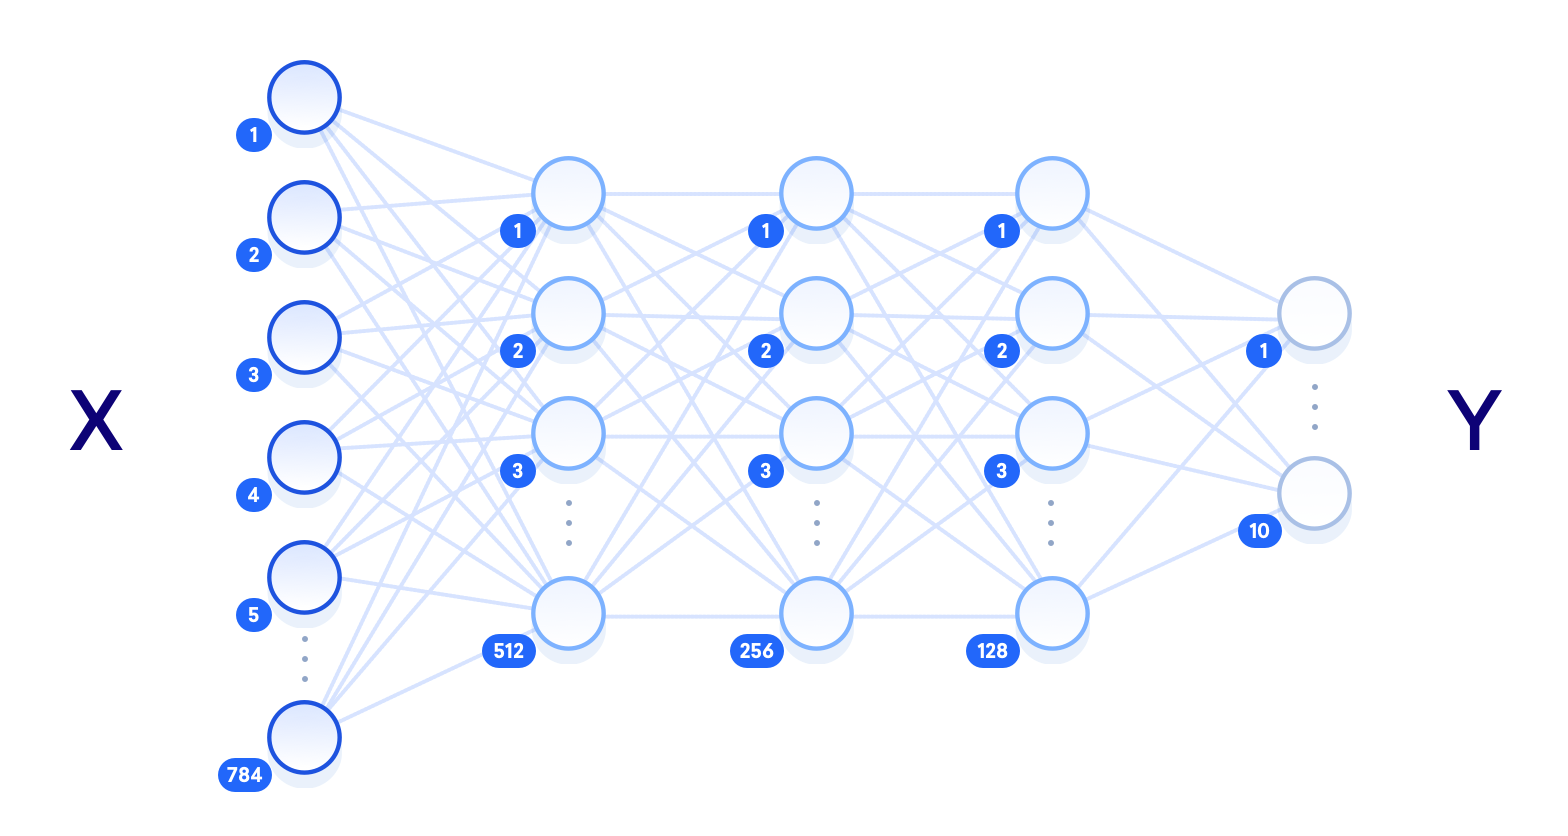
\includegraphics[width=0.7\textwidth, angle=0]{cnwitLM.png}	
	\caption{An example of a possible architecture \citep{digitaloceanBuildNeural}} 
	\label{MNIST}%
\end{figure}

The choices above were selected as they tend to be the most popular choices of activation functions, optimizers and loss functions. The different number of hidden layers used will be $1, 2$ and $3$, with the number of nodes in these layers being either $10, 50$ and $100$. All the hidden layers will have the same number of hidden nodes. This is because there are already $72$ different neural network possibilities to run through which is computationally expensive to run. A further extension to the investigation could include different pyramid architectures.

For simplicity, our final layer will use the softmax activation function. The softmax activation function is a normalized exponential function that converts $m$ real numbers into a probability distribution with $m$ possible outcomes. In particular, this is useful for predicting class probabilities from a neural network's output:
$$
\operatorname{Softmax}(X)=\frac{e^X}{\sum_{i=1}^m e^{X_i}}
$$

The number of epochs in the neural network can also affect accuracy. This  is a hyperparameter that defines the number times that the learning algorithm will work through the entire training dataset. Setting one epoch means each sample has had an opportunity to update the internal model parameters. For the purposes of this investigation, the number of epochs has been set to $5$, although will be changed in the overfitting analysis. Increasing epoch analysis will exponentially increase the number of models that have to be run so is beyond the scope of this investigation.

\section{Evaluation of Models}

As a baseline model to compare against, a simple pyramid architecture is run.
This has 784 input nodes followed by a ReLU hidden layer of $20$ nodes and a second hidden layer of $15$ nodes. Finally there is an output layer with $10$ nodes using the softmax activation function. This model attained an accuracy of $90.35\%$. Although this seems like a good accuracy, in reality $1$ in $10$ images are incorrectly labelled which is a poor performance for real-life applications.
% Best architecture:
% ((3, 100, 'adam', 'categorical_crossentropy', 'relu'), 0.9709)
\subsection{Model Performance}

After running all $72$ neural networks, the architectures were ranked in order of their accuracies. The full table is available within the accompanying notebook.

\subsubsection{Best and Worst Models}

The top 10 best performing models as shown in Figure \cref{best} have similar trends. The best performing model has an accuracy of $97.10\%$, which is almost perfect accuracy and outperforms the baseline model by almost $7\%$.

All of the models use the `Adam' optimiser and use the `ReLU' activation function. This indicates that for the MNIST dataset in particular, these are the best parameters to use. The top $5$ models use categorical crossentropy as a loss function indicating this is the best loss function. The architecture of the top $2$ performing architectures have $3$ hidden layers, and none of the top $10$ have $10$ nodes in their hidden layers, implying more hidden nodes perform better.

The worst performing models are shown in Figure \cref{worst}. The accuracies were much lower than anticipated, with accuracies as low as $7.22\%$, which is $90\%$ worse than the best performing model. The model performs worse than guessing as there would be an on average $10\%$ accuracy guessing correctly given there are only $10$ classes. This indicates the neural network architecture is incredibly poor for the dataset. 


All but one of the models use the mean absoulte error as a loss function, which indicates this performs particularly badly. This is a similar case for the sigmoid activation function. All the optimizers in the bottom $10$ are the Stochastic Gradient Descent model, also indicating its poor performance in this scenario. There are many different layers and nodes within the hidden layers in the bottom $10$. However there is a trend towards fewer hidden nodes. This indicates the number of hidden nodes and number of layers did not have a large effect on the accuracy compared to some other parameters, but are useful for fine tuning the architecutre.

\subsubsection{Possible explanations of results}

One of the largest differentiating factors between the best and worst models is the activation function. ReLU performs well and sigmoid performs poorly in contrast. A possible reason of this is the sigmoid function has pushed the values to the extremes of $0$ and $1$. This may have negatively affected the result to a large extent, particularly when compounded over several layers and during backpropagation. ReLU, in contrast, maintains a varied amount of values, unless the weights given are negative. Within image recognition, the sigmoid function is not often used for this reason. A potential further investigation is to see if the variant Leaky ReLU performs better, as negative values are instead assigned the value $0.1x$ instead of $0$.

\begin{figure}[h]
	\centering 
	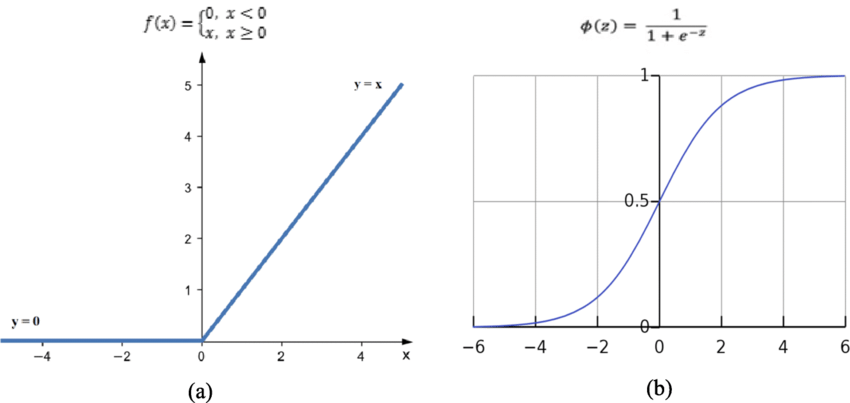
\includegraphics[width=0.7\textwidth, angle=0]{a-ReLU-activation-function-b-Sigmoid-function.png}	
	\caption{ReLU (left) and Sigmoid (right) \citep{article}} 
	\label{best}%
\end{figure}

Another key factor was the choice of optimizer. Adam is a more sophisticated variant of SGD which is a potential reason it performed better. Within its algorithms, there are further considerations such as adaptive learning rates for each parameter, momentum and squared gradient evaluation to converge faster and handle noisy gradients, and bias correction to improve stability. For the choice of loss function, categorical crossentropy performs well on classification problems utilising probabilities, compared to mean absolute error which is better for regression problems, making it more unsuitable for our data. 

Within Neural Networks, overfitting and underfitting can occur which will affect outputs from the network. Overfitting is the phenomenon when the network is adapted too closely to the seen data, and so does not generalize
to unseen data. Underfitting is the opposite, in which the network does not take enough information from the training data so does not predict test data well. A way to investigate this is to use a validation method. Some of the training data is unused so that it can be used as a validation dataset. This is shown for the best performing model in Figure \cref{bests} and the worst performing in Figure \cref{worsts}.

Figure \cref{bests} shows that initially the model initially underfits the data and then fits the data well after two epochs. This is because initially validation data is more accurate than the training data and once it becomes worse, the accuracies of the training and validation data flatten. In contrast, Figure \cref{worsts} shows a clear case of underfitting. The validation data performs better in both cases and neither graph flattens at the end. In particular, the accuracy graph is the wrong shape, indicating a poor fitting of the model. This is a key reason why the model performed poorly.

\subsection{Hidden Layer Parameter Investigation}

As mentioned earlier, due to the limited variability that could be conducted for the investigation, the effect of the hidden layer size and number of hidden layers could not be observed well. More models were rerun with the optimizer Adam, ReLU as the activation function, and sparse categorical crossentropy as the loss function. 

A varied number of hidden layers were experimented, from $16$ up to $256$ and results were recorded in Figure \cref{layers}. Note, $10$ nodes were used in each layer. Clearly, in our previous investigation, looking at only $3$ hidden layers did not give us a full picture. We can see that the number of hidden layers increases the accuracy of the model, up to $128$ hidden layers, at which it plateaus. This makes $128$ layers optimal for the data set. However it is important to note this is computationally expensive so less hidden layers will compromise accuracy for performance time. The effect of increasing the number of hidden layers increases performance up to $1.4\%$, which is a lot but insignificant when taking into account some other factors. This suggests that altering this parameter is best for fine tuning the model.

Similarly, the number of nodes in the hidden layers were investigated in Figure \cref{nodes} over three hidden layers. This parameter affected the accuracy more than the number of layers, with a difference of $3\%$ between the best and worst accuracies. The best accuracy peaks around $150$ nodes and then decreases again, similar to changing the number of layers. Again, increasing the number of nodes significantly affects the runtime of the network so a compromise must be reached between accuracy and performance time, especially on larger models.

\subsection{Other Methods - CNN}

Whilst standard neural networks managed to achieve an accuracy of over $97\%$, other techniques can also be utilised to increase our accuracies further. One such example is the use of convolutional neural networks (CNNs). These architectures are much more complex and use deeper mathematical techniques. 

The main differences between a CNN and a standard neural network are the use of tensors in the input (n-dimensional matrices) with each entry corresponding to a pixel and its colour (usually red, green and blue values). Additionally, CNNs have a filter called a kernel which is a linear mapping from a tensor to a matrix to determine the features. 

Naturally, there are layers known as convolutional layers that are linked to previous layers using a unique kernel. These convolutional layers are based on the mathematical idea of convolutions: $(f * g)(t) = \int_{-\infty}^{\infty} f(\tau) \cdot g(t - \tau) \, d\tau$. In a convolutional layer, various different kernels or convolutions are applied to the image. Convolutional layers are often combined with pooling layers. In a pooling layer, a few entries  are combined into one entry, either by taking the maximum (max pooling) or by averaging. Usually at the end, there is a flattening layer that creates the output from the matrices. 

Figure \cref{VGG} shows an example of a CNN architecture that can be used. It is known as a `Tiny VGG' architecture, based on a more complex VGG architecture often used in image recognition.  All activation functions used are ReLU for the convolutional layers, with the final dense layer being a final perceptron layer with $10$ outputs using the softmax activation layer as before.

\begin{figure}[htb]
	\centering 
	\includegraphics[width=0.9\textwidth, angle=0]{VGG.png}	
	\caption{Tiny VGG architecture - an example of a CNN \citep{mediumStartedWith}} 
	\label{VGG}%
\end{figure}

When running the architecture on the MNIST dataset, we obtain an accuracy of $98.93\%$. This is the best accuracy out of all the neural networks tested.

\section{Conclusion}

In conclusion, for image recognition, the parameters chosen in the architecture of the neural network drastically effect the final accuracy. The most important factors are activation functions and optimizers. In our case, using the MNIST dataset for digit recognition, the sigmoid function performed particuarly badly. The Adam optimizer and ReLU activation function consistently performed well. When choosing a loss function, consideration of the final output layer is important. In our case, as there were $10$ possible outputs, crossentropy worked well as it handled categorical data better, whereas mean absolute error performed poorly. In other cases, where there are only two outputs, mean absolute error may perform better. The number of hidden layers and the number of nodes (depth) in each are less important, but when fine tuning the architecture it can increase the accuracy of the model.


Whilst simple neural networks as used give excellent results for image recognition, newer more sophisticated methods can result in even better accuracies, such as the use of Convolutional Neural Networks, although the parameters and hyperparameters of these must also be chosen wisely.

\section{Figures}
Below are figures referenced within the evaluation.

\begin{figure}[h]
	\centering 
	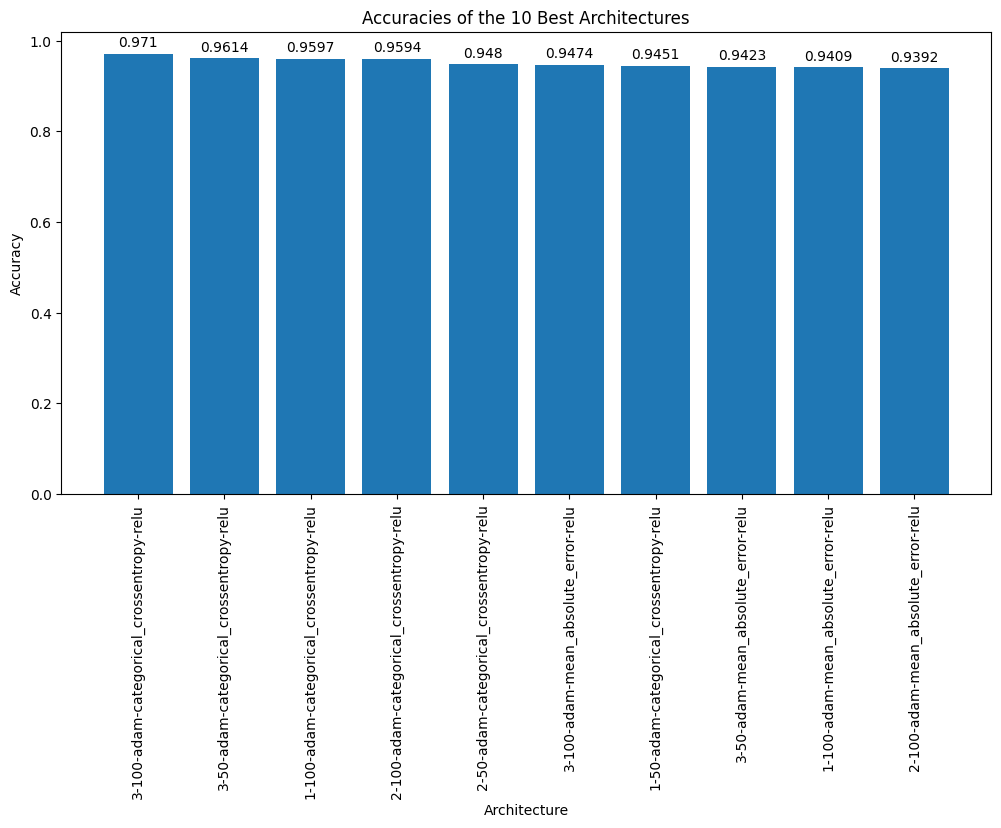
\includegraphics[width=0.86\textwidth, angle=0]{best.png}	
	\caption{The top 10 best performing architectures, with their respective accuracies written above the bars. The labels are written as: number of hidden layers - number of nodes in hidden layers - optimizer - loss function - activation function.} 
	\label{best}%
\end{figure}

\begin{figure}[h]
	\centering 
	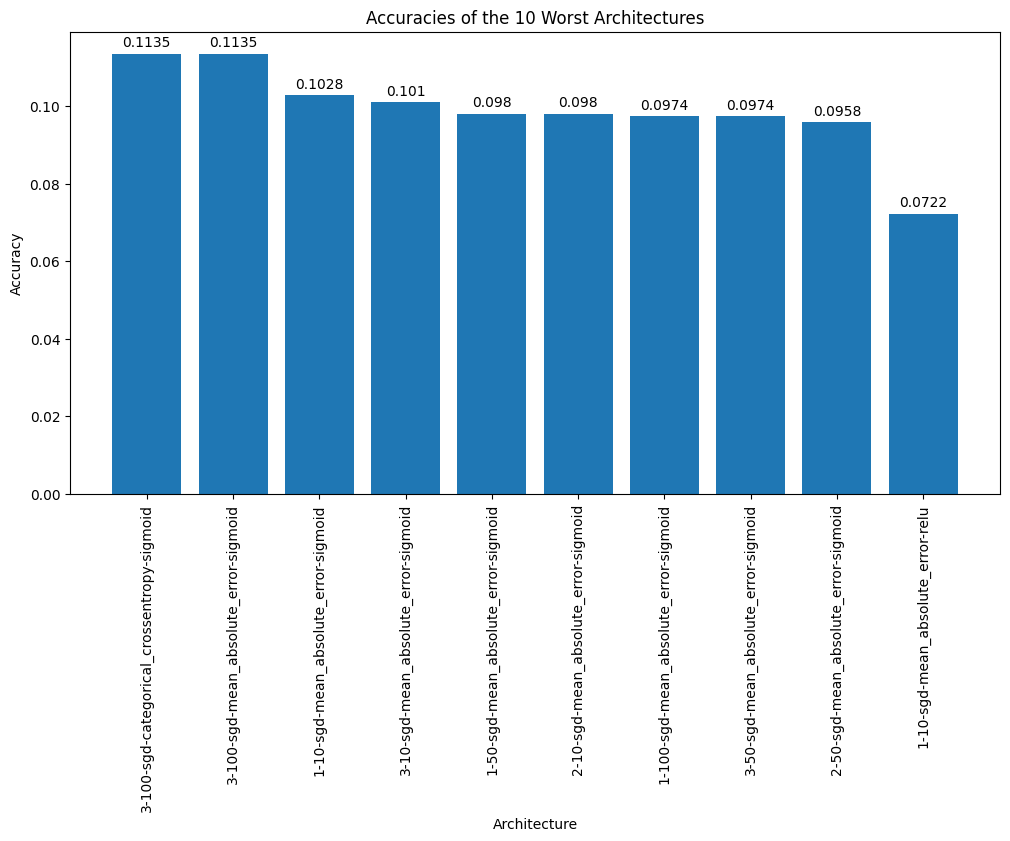
\includegraphics[width=0.86\textwidth, angle=0]{worse.png}	
	\caption{The top 10 worst performing architectures, with their respective accuracies written above the bars. The labels are written as: number of hidden layers - number of nodes in hidden layers - optimizer - loss function - activation function.} 
	\label{worst}%
\end{figure}

\begin{figure}[h]
	\centering 
	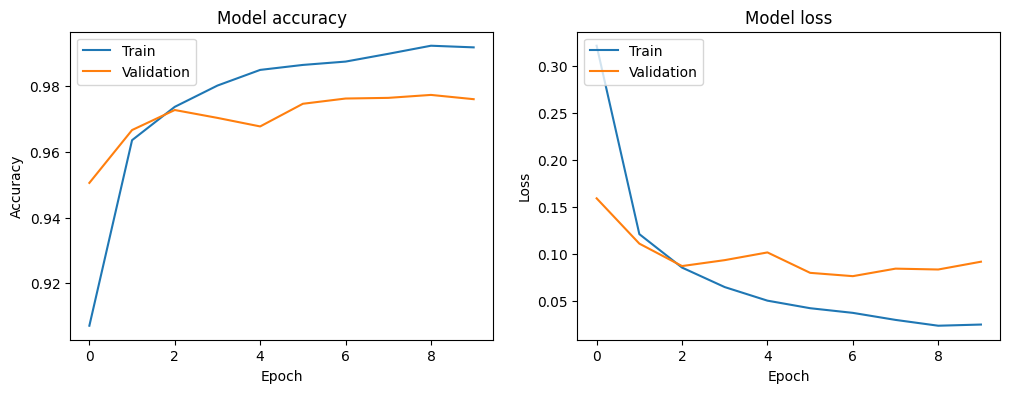
\includegraphics[width=1\textwidth, angle=0]{bests.png}	
	\caption{Model Valuation of the Best Architecture} 
	\label{bests}%
\end{figure}

\begin{figure}[h]
	\centering 
	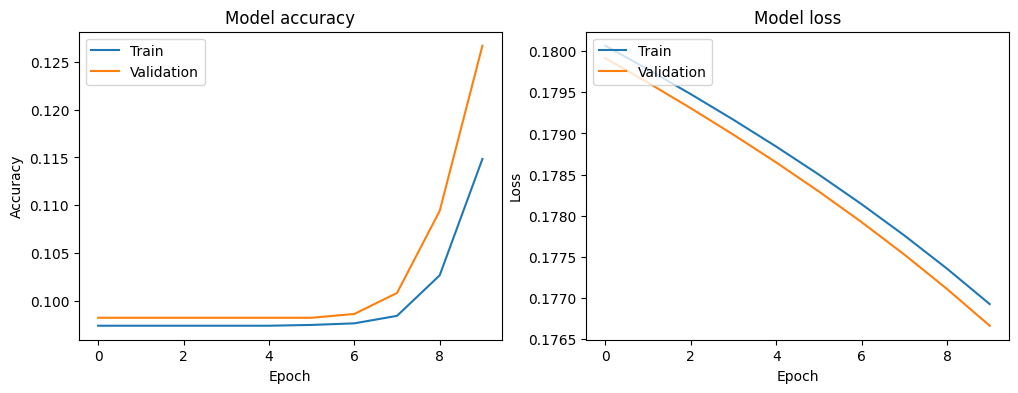
\includegraphics[width=1\textwidth, angle=0]{worsts.png}	
	\caption{Model Valuation of the Worst Architecture} 
	\label{worsts}%
\end{figure}

\begin{figure}[h]
	\centering 
	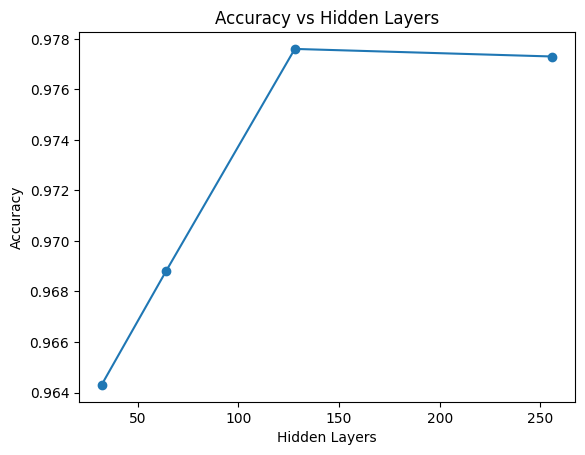
\includegraphics[width=0.8\textwidth, angle=0]{layers.png}	
	\caption{Graph showing how accuracy changes over different hidden layers.} 
	\label{layers}%
\end{figure}

\begin{figure}[h]
	\centering 
	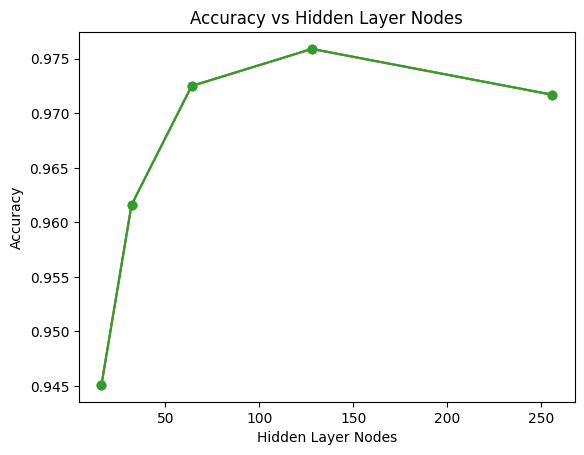
\includegraphics[width=0.8\textwidth, angle=0]{nodes.png}	
	\caption{Graph showing how accuracy changes over different numbers of nodes in hidden layers.} 
	\label{nodes}%
\end{figure}

\clearpage
\bibliography{references}

% \nocite{*} % used if you want to include everything in the bibliography even if they were never used.
\end{document}
